\beginsong{Weberlied}[
    txt={Heinrich Heine}, 
    txtjahr={1844},
    mel={helm (Helmut König)}, 
    bo={196}, 
    pfii={50}, 
    pfiii={24}, 
    gruen={156}, 
    kssiv={32}, 
    siru={122}, 
    tonspur={336}, 
    index={Im düsteren Auge keine Träne}
]

\beginverse*
{\nolyrics Intro: \[Em] \[C] \[D] \rep{2}}\newline
\endverse

\beginverse
\endverse
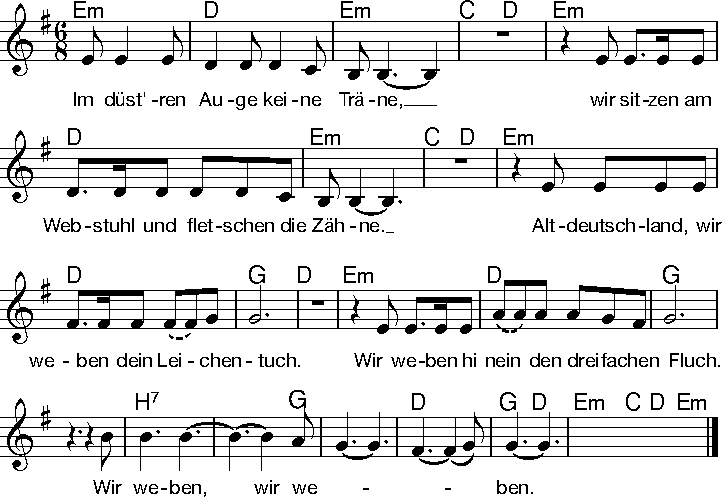
\includegraphics[draft=false, width=1\textwidth]{Noten/Lied027.pdf}	

\beginverse\memorize
\[Em]Ein Fluch dem \[D]Gotte zu dem wir ge\[Em]beten \[C] \[D]
\[Em]in Winters\[D]kälte und Hungers\[Em]nöten. \[C] \[D]
\[Em]Wir haben ver\[D]gebens gehofft und ge\[G]harrt. \[D]
\[Em]Er hat uns ge\[D]äfft, gefoppt und ge\[G]narrt.
\endverse

\beginchorus
Wir \[H7]weben, wir \[Em]we \[D]- \[G]ben. \[D] \[Em] \[C] \[D] \[Em] \[C] \[D]
\endchorus

\beginverse
^Ein Fluch dem ^König, dem König der ^Reichen, ^ ^
^den unser ^Elend nicht konnte er^weichen, ^ ^
^der den letzten ^Groschen von uns er^presst ^
^und uns wie ^Hunde erschießen ^lässt.
\endverse

\printchorus

\beginverse
^Ein Fluch dem ^falschen Vater^lande, ^ ^
^wo nur ge^deihen Schmach und ^Schande, ^ ^
^wo jede ^Blume früh ge^knickt, ^
^wo Fäulnis und ^Moder den Wurm er^quickt.
\endverse

\printchorus

\beginverse
^Das Schifflein ^fliegt, der Webstuhl ^kracht. ^ ^
^Wir weben ^emsig Tag und ^Nacht. ^ ^
^Altdeutschland wir ^weben dein Leichen^tuch, ^
^wir weben hi^nein den dreifachen ^Fluch.
\endverse

\printchorus

\endsong

\beginscripture{}
Das Lied beschreibt das Elend der schlesischen Weber, die 1844 im Zuge der Industrialisierung zum Protest gegen Ausbeutung und Lohnverfall einen Aufstand organisierten. Es wurde zuerst in Karl Marx' Flugschrift ''Vorwärts!'' veröffentlicht. Das Königlich Preußische Kammergericht verbot das Gedicht und seine Rezitation bei Gefängnisstrafe.
\endscripture
